\begin{frame}{Reflector gain depends on the readout geometry}
\begin{center}
\begin{tabular}{lll}
\toprule
Configuration & Metal / dielectric END yield & Comparison\\
\midrule
END-only & $\EndGain\pm\EndGainSem$ & \IdDZero/\IdDThree\\
EndTop & $\EndTopGain\pm\EndTopGainSem$ & \IdBZero/\IdAZero\\
Ratio of those gains & $\GainRatio\pm\GainRatioSem$ & factorial contrast\\
\bottomrule
\end{tabular}
\end{center}
\begin{block}{The guard is already corrected in these comparisons}
The reflector is the changed optical choice within each readout geometry. A single multiplicative ``reflector correction'' does not describe both geometries.
\end{block}
Ratio uncertainties retain the historical zero-covariance approximation; using the same seeds does not supply an estimated covariance.
\Source{\FactorSource}
\end{frame}

\begin{frame}{Many more encounters accompany a modest END-yield gain}
\begin{center}
\begin{tabular}{lcc}
\toprule
END-only factory & Air $\to$ wrap encounters / started optical photon\\
\midrule
Dielectric, \IdDThree & $\MultiplicityDielectric$\\
Metal, \IdVOne & $\MultiplicityMetal$\\
\bottomrule
\end{tabular}
\end{center}
\begin{block}{Measured: about $\EncounterRatio\times$ more forward encounters}
Encounters include outcomes other than reflection. These are unconditional all-optical means, not means per scintillation photon and not counts of successful bounces.
\end{block}
\textbf{Limited interpretation:} specular reflection preserves the incidence angle for equal or parallel face normals. Recycling need not restore TIR acceptance at those faces. Orthogonal faces differ; no angular-history study was performed.
\Source{\CommonSource\ END-only, $N_{\rm TOP}=\NoTopCount$, $x=\Zero\mm$, $N=\MainN$/arm, \MetalWorkers\ workers/eventModulo \One. \IdDThree/\IdVOne: \texttt{\ShaDThree}/\texttt{\ShaVOne}. Sidecars: \texttt{sources/multiplicity\_dielectric}, \texttt{sources/multiplicity\_metal}.}
\end{frame}

\begin{frame}{EndTop: the reflector gain grows toward the ends}
\begin{center}
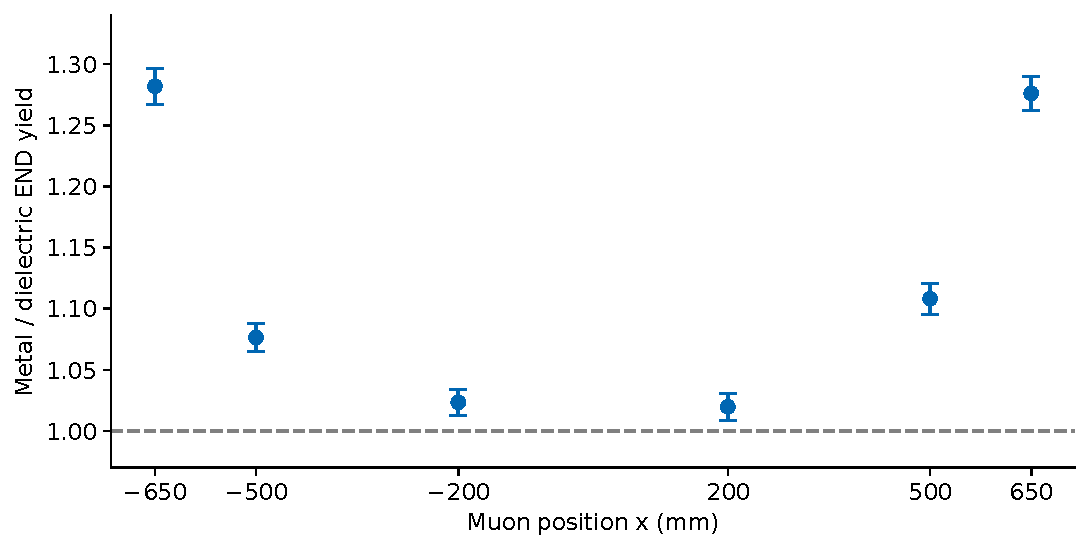
\includegraphics[width=\FullFigureWidth,height=\FigureHeight,keepaspectratio]{figs/position_gain.pdf}
\end{center}
The comparison uses the same readout layout and a corrected guard in both arms. Error bars are the recorded approximate ratio SEMs.
\Source{\CommonSource\ EndTop, $N_{\rm TOP}=\TopCount$; $x\in\{\pm\XNear,\pm\XMiddle,\pm\XFar\}\mm$; $N=\ScanN$/arm/position, one worker. Dielectric/metal commits: \texttt{\ShaAZero}/\texttt{\ShaBZero}. Sidecars: \texttt{sources/positions}, \texttt{figs/position\_gain}. Per-cell commands: \texttt{sources/provenance.json}.}
\end{frame}
